\documentclass[conference, 10pt]{IEEEtran}
%\IEEEoverridecommandlockouts
% The preceding line is only needed to identify funding in the first footnote. If that is unneeded, please comment it out.
\usepackage{cite}
\usepackage{amsmath,amssymb,amsfonts}
\usepackage{algorithmic}
\usepackage{graphicx}
\usepackage{textcomp}
\usepackage{xcolor}
\usepackage[colorlinks = true,
            linkcolor = blue,
            urlcolor  = blue,
            citecolor = blue,
            anchorcolor = blue]{hyperref}
\usepackage[spanish,activeacute]{babel}

\def\BibTeX{{\rm B\kern-.05em{\sc i\kern-.025em b}\kern-.08em
    T\kern-.1667em\lower.7ex\hbox{E}\kern-.125emX}}
\begin{document}

\title{Predicción del precio de bolsa de energía eléctrica Del Mercado Energía Mayorista Colombiano}

\author{\IEEEauthorblockN{Andrea Margarita Beleño}
\IEEEauthorblockA{200620739\\
E-mail:a.beleno@uniandes.edu.co}
\and
\IEEEauthorblockN{María Valeria Gaona}
\IEEEauthorblockA{202214418\\
E-mail:mv.gaona@uniandes.edu.co}
}

\maketitle

\begin{abstract}
El precio de bolsa de energía eléctrica del Mercado de Energía Mayorista (MEM) Colombiano está dado por diversos factores para generar un ambiente propicio de competencia y formación eficiente de precios, que le permitan a la demanda tener precios óptimos. Es por ello que es fundamental el análisis  de este mercado para que a medida que pase el tiempo, los agentes que participan en este mercado puedan identificar factores de riesgo más rápido y así, tomar las mejores decisiones para la economía y distribución de energía del país. Por lo tanto, de acuerdo con el análisis anterior, contar con una herramienta como una aplicación web que pueda predecir este valor genera una dinámica más eficiente para los agentes que están dentro del sector y a su vez, a ciudadanos que estén interesados en el campo energético. \
Para acceder a la aplicación web, se presenta el siguiente enlace: url{https://aplicaciones-web-abeleno.shinyapps.io/pred_precio_bolsa_horario/} A su vez, el link al  repositorio del presente documento se encuentra en el siguiente enlace: \url{https://github.com/mvgaona/Proyecto-final-MEcA-4107}
\end{abstract}


\section{Introducción}
El mercado eléctrico colombiano es un mercado competitivo en donde participan generadores, transmisores, distribuidores, consumidores y comercializadores de energía. Este mercado se divide en dos segmentos: Corto y largo plazo, sin embargo, en el siguiente documento se presentará el análisis del mercado en corto plazo por medio de la bolsa de energía de Colombia, la cual es administrada por XM, en donde se presenta la participación de generadores y comercializadores de energía para la compra y venta a precio de bolsa de energía eléctrica, con el objetivo de suplir la demanda adecuada de energía en el país.\\
De acuerdo con Trespalacios, Pantoja & Fernandez (2017)[5], el mercado spot o la bolsa de energía hace referencia al mercado en donde se obtiene la energía eléctrica de forma instantánea, con el objetivo de lograr un balance entre oferta  y demanda. A su vez, los autores afirman que dicho precio de bolsa se define mediante un conjunto de normas que buscan precisar el nivel de referencia en caso de escasez.\\
Poveda (2012) [1] afirma que el despacho ideal es el programa de generación que está dado por el uso de los recursos más económicos hasta cubrir la demanda doméstica real, más las Transacciones Internacionales de Electricidad de Corto Plazo - TIE (Exportaciones como demanda e importaciones como generación), más las pérdidas del STN (Sistema de Transmisión Nacional). Teniendo en cuenta lo anterior, el precio de bolsa está dado por el precio de oferta obtenido por medio del despacho ideal, el cual es utilizado para valorar los intercambios en bolsa.\\
El correcto funcionamiento del mercado eléctrico es fundamental para el análisis de la demanda energética en el país: si es necesario realizar estrategias en el manejo de los recursos naturales con los que se genera energía, si la dinámica de compra y venta de energía está siendo óptima para la economía y sociedad colombiana. Generar una proyección de estos precios permite poder hacer inferencia acerca de cómo el mercado puede estar funcionando y aunque ´ este sea un sistema fluctuante, se puede generar predicciones acerca de su comportamiento.\\

En el siguiente documento se encuentra el análisis acerca de los datos recaudados para la predicción del precio de bolsa de energía eléctrica del mercado de energía mayorista colombiano, en donde se implementará un modelo de Machine Learning automático en una aplicación web, que permitirá modelar futuros precios de bolsa y con ello, tomar decisiones comerciales basadas en los datos adquiridos


\section{Datos} \label{AA}

El precio de una vivienda puede estar dado por diferentes factores, tanto económicos como sociales. En el caso Colombiano, estos precios pueden estar influenciados por elementos propios de la vivienda y a su vez, por elementos geoespaciales, como la distancia a diversos lugares públicos (Bares, transporte público, etc). Para realizar un modelo de predicción de precios de la vivienda, es necesario contar con las variables determinantes y relevantes del precio, para que este modelo sea robusto, pero no se incurran en gastos que entorpezcan esta labor. En el presente modelo de predicción se tomó en cuenta solo los datos de  las viviendas ubicadas en las localidades objetivo (Chapinero y Poblado) y el total de datos (Base de entrenamiento y base de testeo) es de 24.843 viviendas. \
Dentro del proceso de recolección de datos puede ocurrir que no se encuentre toda la información necesaria, ya sea porque la base de datos no provee dicha información o, por el contrario, no se pudo recolectar toda la información de cada vivienda. Es por eso que es necesario realizar un proceso de limpieza y recuperación de datos. Se realizaron diversos procesos para poder contar con toda la información:\\ 
-Se cuenta con variables las cuales ya tienen la información completa, por lo tanto no es necesario realizar ningún tratamiento:
\begin{itemize}
\item \textit{Ubicación}: La ubicación del inmueble en el modelo será esencial para el análisis ya que se analizarán dos localidades de dos ciudades diferentes y los precios de las ciudades si bien están dados por características similares, el costo de vida por ciudad también influye en el valor de la vivienda. Esta variable es categórica, y se tiene que la mayoría de datos son de la ciudad de Bogotá (ver Cuadro ~\ref{tab_1}).
\item \textit{Tipo de propiedad}: Si la propiedad es un apartamento o si es una casa influye sustancialmente en el precio, ya que el área de una casa suele ser más grande, cuenta con más oportunidad de reformas y espacios más amplios de esparcimiento. Esta variable categórica cuenta con una mayor proporción de apartamentos (Ver Cuadro ~\ref{tab_2}).
\end{itemize}
-Para algunas variables existentes en la base de datos, se generó la comparación entre dicha información y los valores hallados por medio de la inspección de la descripción de cada inmueble, generando las siguientes variables sin información faltante:
\begin{itemize}
\item \textit{Habitaciones}: El número de habitaciones de la vivienda es determinante en el precio de la misma, ya que se puede contar con un aproximado del espacio y de cuántos individuos pueden vivir, es decir, entre más habitaciones, el precio del inmueble tiende a incrementarse. Por lo tanto, dentro del análisis descriptivo de este predictor se encuentra que es  una variable numérica, con media de 3 habitaciones (Ver Cuadro ~\ref{tab_3}).
\item \textit{Cantidad de baños}: Este es otro factor de decisión importante en el precio del inmueble, ya que sin baños, los individuos no pueden satisfacer las necesidades básicas de aseo. Por lo tanto es necesario contar con al menos un baño y con ello, se puede identificar que a medida que aumentan la cantidad de baños, el precio de igual manera se verá afectado e incrementará. De acuerdo con lo anterior, se observa que en la variable numérica, la media fue de 3 baños (ver Cuadro ~\ref{tab_4}).
\end{itemize}

-De acuerdo con la información proporcionada por la descripción de cada inmueble, se generaron las siguientes variables:

\begin{itemize}
\item \textit{Ascensor}: Si el inmueble cuenta con ascensor o no es determinante en el caso de los apartamentos de pisos altos, es por eso que se considera un predictor importante del modelo, ya que quienes viven en pisos más altos, buscan apartamentos donde tenga ascensor y a su vez, el precio aumenta si el inmueble cuenta con este. Dentro del análisis descriptivo de la variable, es posible identificar que es una variable dicótoma, donde 1 corresponde a si el inmueble cuenta con ascensor y 0 si no (Ver Cuadro ~\ref{tab_5}).Los inmuebles que no cuentan con ascensor también pueden ser apartamentos que no cuentan con uno y casas que no lo necesitan.
\item \textit{Parqueadero}: En la actualidad, gran parte de los individuos cuentan con uno o más carros, por lo tanto, es necesario que el inmueble cuente con al menos un parqueadero, por lo tanto, si el inmueble incluye al menos un garaje, el precio de la vivienda tenderá a aumentar su valor. Por otra parte, de acuerdo con el análisis descriptivo, se identifica que esta es una variable dicótoma, en donde 1 hace referencia a que la casa o el apartamento cuenta con al menos un parqueadero y 0 que no lo hace. La proporción de inmuebles que cuentan con al menos un parqueadero es que la mayoría de inmuebles de la base no cuenta con parqueaderos (ver cuadro ~\ref{tab_6}). La proporción puede estar dada debido a que algunos vendedores no ofrecieron dicha información, por ejemplo.
\end{itemize}
 
-De acuerdo con la ubicación geoespacial, se pueden recuperar datos por medio de la búsqueda de características similares de otras viviendas y dicho promedio, adjuntarlo al inmueble que no cuenta con información, ya que al estar en un perímetro cercano, los inmuebles suelen presentar características similares.
\begin{itemize}
\item \textit{Área}: El área de un inmueble es fundamental para conocer el precio del mismo, ya que a medida que el área aumente, también el precio. Esto se da debido a que un espacio amplio permite contar con un mayor número de habitaciones, baños, una cocina más amplia y demás espacios de esparcimiento. Además, permite más posibilidades de remodelación y de inversión. Por lo tanto, ante la variable numérica presentada, se encuentran que se tiene una media de 286 m2. Para más información (ver Cuadro ~\ref{tab_7})

\end{itemize}

-Por medio de la ubicación geoespacial, las variables adicionales que se encontraron y que consideramos relevantes para la predicción, fueron las siguientes: 
\begin{itemize}
\item \textit{Distancia a Transporte público}: Contar con al menos un transporte público cerca de la vivienda es fundamental para poder desplazarse con facilidad. Por lo tanto, esta variable presenta la distancia mínima que tiene el inmueble con al menos un medio de transporte público, ya que a medida que esta distancia sea más corta, el precio puede incrementarse. Para esta variable se cuenta con una media de 1,5km (Ver Cuadro ~\ref{tab_8})
\item \textit{Distancia a Bares}: La distancia mínima a bares es otro factor a tener en cuenta, ya que, en general, este tipo de establecimiento hace que pueda generar incomodidad a los habitantes en las horas de la noche. Por lo tanto, al estar cada vez más alejados de un bar, el comprador puede estar más interesado en el inmueble. De acuerdo con la variable numérica, se presenta que la media de distancia se encuentra en 694m (Ver Cuadro ~\ref{tab_9}).
\item \textit{Distancia a Parques}:La distancia mínima a por lo menos un parque es otro predictor relevante dentro del modelo, ya que, en general, los individuos buscan tener un espacio verde y de recreación cerca, por tema de hijos o mascotas, o porque los compradores también desean un espacio al aire libre para su propio entrenamiento. Por lo tanto, a medida que esta distancia va disminuyendo, el precio del inmueble tiende a incrementar. Esta variable numérica tiene una media de 230m (Ver Cuadro ~\ref{tab_10}). 
\end{itemize}




\section{Modelo}
Con base en las variables presentadas en la sección \ref{AA}, se procedió a realizar varios modelos para determinar cuál era el más apropiado para realizar la predicción de precio de viviendas. Se analizó la posibilidad de partir la base \textit{train} (con 13.693 datos)en un \textit{subtrain} y \textit{subtest}, sin embargo, teniendo en cuenta que la base de \textit{test} original cuenta con 11.150 observaciones, realizar la subdivisión de \textit{train} en un menor número de muestras, podría ir en perjuicio de la predicción por contar con un menor número de datos para entrenar, por lo cual, se decidió implementar los modelos sobre la base \textit{train}. En primera instancia, se realizó una prueba utilizando las 10 variables mencionadas en la sección \ref{AA} y se realizó un modelo de regresión con \textit{OLS} (modelo 1), luego, se realizó la regularización de Lasso para la regresión OLS (modelo 2). Adicionalmente, se realizaron los modelos \textit{Random Forest} (modelo 3) y \textit{XGBoost} (modelo 4), teniendo en cuenta las variables mencionadas anteriormente, para explorar si estas alternativas para datos no lineales podían dar un mejor resultado. Las 10 variables utilizadas para realizar los modelos mencionados anteriormente son las siguientes: 
\begin{itemize}
\item \textit{Ubicación}, \textit{Tipo de vivienda}, \textit{Habitaciones}, \textit{Baños}, \textit{Área}, \textit{Distancia a bares}, \textit{Distancia a transporte público}, \textit{Ascensor}, \textit{Parqueaderos}, \textit{Distancia a parques}.  
\end{itemize}

Luego de correr los modelos, se decidió disminuir el número de variables para realizar las regresiones para los 4 modelos mencionados anteriormente, utilizando 5 variables que se mencionan a continuación: 
\begin{itemize}
\item \textit{Habitaciones}, \textit{Baños}, \textit{Área}, \textit{Distancia a bares}, \textit{Distancia a transporte público} 
\end{itemize}
Se obtuvieron las variables relevantes en el modelo \textit{Random Forest}, que son las 6 que se presentan a continuación :
\begin{itemize}
\item \textit{Habitaciones}, \textit{Baños},\textit{Área}, \textit{Distancia a bares}, \textit{Distancia a transporte público},  \textit{Distancia a parques}
\end{itemize}
Utilizando las variables presentadas anteriormente, se corrieron los modelos mencionados incialmente (\textit{OLS}, \textit{Lasso}, \textit{Random Forest}, \textit{XGBoost}, para un total de 12 modelos. El parámetro de comparación entre modelos fue el RMSE. Se observó que al disminuir la cantidad de variables, el RMSE aumentó, por lo cual, se decidió realizar la comparación con los 4 modelos descritos anteriormente en términos de RMSE. Al hacer la comparación, se obtuvo que el modelo de \textit{Random Forest} con un número de árboles igual a 5, fue el de menor RMSE (este resultado se presenta en la Figura ~\ref{fig_3}). \\
Ahora bien, existen un tema relevante a tener en cuenta para decidir cuál modelo se debe escoger para realizar la predicción, como lo es la relación de dinero para compra (\$) vs. la cantidad de viviendas compradas ($Viv$) (no solo en términos de RMSE), en donde se escoge el modelo con el que se obtenga la menor relación, teniendo en cuenta que entre más casas compradas y menor valor gastado, la relación $ \$/Viv$ será menor. Se realizó la comparación de cada set de modelos, con las 10, 5 y 6 variables, de lo cual se obtuvo la información presentada en los Cuadros ~\ref{tab_11}, ~\ref{tab_12} y ~\ref{tab_13}. Lo anterior, para concluir que el mejor modelo para realizar la predicción fue el de \textit{Random Forest} con 10 variables. Cabe anotar que la cantidad de árboles contemplada para el modelo fue de 5, por lo cual, se decidió entrenar el modelo variando el número de árboles, aumentándolo para disminuir el RMSE; después de intentar varios valores, se decidió fijar el número de árboles en 1.000 (el número de predictores por default fue el $\sqrt{p}$); para este caso, se obtuvo un menor RMSE, y al realizar el cálculo de relación dinero gastado vs viviendas compradas, también fue el más eficiente. Finalmente, la predicción obtenida se guardó en el archivo .csv solicitado.

\begin{figure}[htbp]
\centerline{\includegraphics[width=0.2\textwidth]{../Vistas/Comp_MSE_modelos_var_10.png}}
\caption{Comparación RMSE modelos para obtener \textit{price}}
\label{fig_3}
\end{figure}


\section{Resultados}
Para implementar el modelo en una aplicación web, utilizamos el paquete de \textit{Shiny} de R con los códigos especiales para que sean ejecutados mediante una página web. Para la implementación, se guardaron los modelos que menor RMSE tuvieron para cada modelo de precio horario y estos son los que se ejecutan en la página para la visualización e ingreso de variables por parte de un usuario. En la Figura ~\ref{fig_3} se muestra el entorno de la aplicación web de acceso público pero con limitación en el tiempo, con posibilidad de variar los campos a criterio y conocimiento del usuario. 

\begin{figure}[htbp]
\centerline{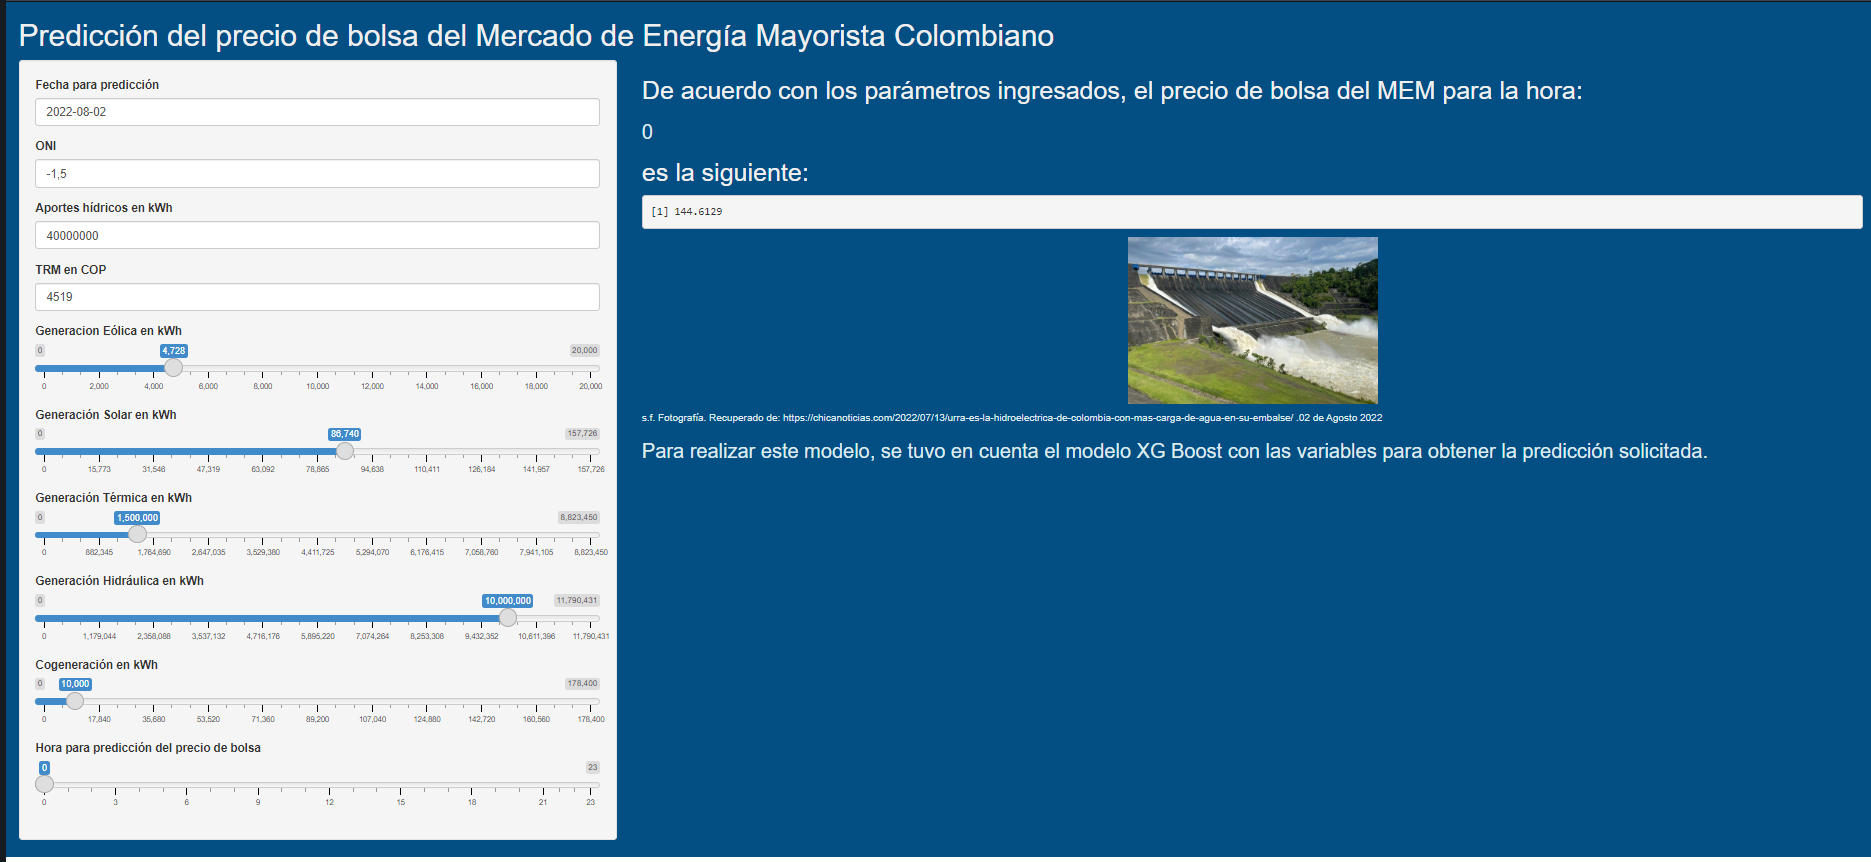
\includegraphics[width=0.2\textwidth]{../Images/Resultado_Trabajo_final.png}}
\caption{Resultado de la aplicación web}
\label{fig_3}
\end{figure}

\section{Conclusiones y recomendaciones}
\begin{itemize}
\item La adquisición de información del texto de descripción es muy dependiente de patrones fijos que permitan extraer los datos de interés fácilmente, por ello, es posible que haya faltado información para tener la información completa de los datos.
\item Fue un bastante interesante obtener los datos geográficos para utilizarlos como predictores o para imputar datos de variables existentes, fue en la parte del PS3 que más se demoró para obtener y que representó un gran reto y esfuerzo, sin embargo, consideramos la información obtenida muy relevante y que puede servir para futuras aplicaciones.
\item Los resultados más aceptables para el ejercicio fueron los que tuvieron en cuenta mayor cantidad de variables para obtener la predicción.
\item Para el presente trabajo, el modelo con menor RMSE y que también presentó una menor relación precio vs vivienda, fue el escogido para realizar la predicción y fue el que se entrenó posteriormente para obtener la predicción.
\item Como recomendación, con mayor cantidad de tiempo, se hubiese podido realizar otros modelos variando los hiperparámetros del modelo \textit{XGBoost}. 

\end{itemize}

\appendix[Cuadros de Variables descriptivas]
Se presentan los Cuadros donde se consignan las estadísticas descriptivas de las variables explicadas en la sección \ref{AA}.\\ 
\begin{table}[htbp]
\caption{Cuadro descriptivo \textit{Ubicación}}
\begin{center}
\begin{tabular}{|c|c|}
\hline
\multicolumn{2}{|c|}{\textbf{Ubicación}} \\
\cline{1-2} 
\hline
 Bogotá D.C.&Medellín\\
 14.244&10.599\\
 (57,34\%)&(42,7\%)\\
 
	\hline
\end{tabular}
\label{tab_1}
\end{center}
\end{table}

\begin{table}[htbp]
\caption{Cuadro descriptivo \textit{Tipo de vivienda}}
\begin{center}
\begin{tabular}{|c|c|}
\hline
\multicolumn{2}{|c|}{\textbf{Tipo de Vivienda}} \\
\cline{1-2} 
\hline
 Casa&Apartamento\\
 2.038&22.805\\
 (8,2\%)&(91,8\%)\\
 
	\hline
\end{tabular}
\label{tab_2}
\end{center}
\end{table}

\begin{table}[htbp]
\caption{Cuadro descriptivo \textit{Habitaciones}}
\begin{center}
\begin{tabular}{|c|c|c|c|}
\hline
\multicolumn{4}{|c|}{\textbf{Habitaciones}} \\
\cline{1-4} 
\hline
 Mín&Media&Máx.&Moda\\
\hline
 1&3&11&3\\
 	\hline
\end{tabular}
\label{tab_3}
\end{center}
\end{table}

\begin{table}[htbp]
\caption{Cuadro descriptivo \textit{Número de baños}}
\begin{center}
\begin{tabular}{|c|c|c|c|}
\hline
\multicolumn{4}{|c|}{\textbf{Número de baños}} \\
\cline{1-4} 
\hline
 Mín&Media&Máx.&Moda\\
\hline
 1&3&13&2\\
 	\hline
\end{tabular}
\label{tab_4}
\end{center}
\end{table}

\begin{table}[htbp]
\caption{Cuadro descriptivo \textit{Ascensor}}
\begin{center}
\begin{tabular}{|c|c|}
\hline
\multicolumn{2}{|c|}{\textbf{Ascensor}} \\
\cline{1-2} 
\hline
 Tiene ascensor&No tiene ascensor\\
 19.388 (78,04\%)&5.455(21,96\%)\\
  
	\hline
\end{tabular}
\label{tab_5}
\end{center}
\end{table}

\begin{table}[htbp]
\caption{Cuadro descriptivo \textit{Parqueadero}}
\begin{center}
\begin{tabular}{|c|c|}
\hline
\multicolumn{2}{|c|}{\textbf{Parqueadero}} \\
\cline{1-2} 
\hline
 Tiene parqueadero&No tiene parqueadero\\
 7.885(31,74\%)&16.958(68,26\%)\\
  
	\hline
\end{tabular}
\label{tab_6}
\end{center}
\end{table}

\begin{table}[htbp]
\caption{Cuadro descriptivo \textit{Área}}
\begin{center}
\begin{tabular}{|c|c|c|c|}
\hline
\multicolumn{4}{|c|}{\textbf{Área (m\^{2})}} \\
\cline{1-4} 
\hline
 Mín&Media&Máx.&Moda\\
\hline
 74,06&286,75&3.940,14&193,7414\\
 	\hline
\end{tabular}
\label{tab_7}
\end{center}
\end{table}


\begin{table}[htbp]
\caption{Cuadro descriptivo \textit{Transporte Público-TP}}
\begin{center}
\begin{tabular}{|c|c|c|c|}
\hline
\multicolumn{4}{|c|}{\textbf{Distancia TP (m)}} \\
\cline{1-4} 
\hline
 Mín&Media&Máx.&Moda\\
\hline
 4,397&1.519,834&4.472,144&2.168,091\\
 	\hline
\end{tabular}
\label{tab_8}
\end{center}
\end{table}

\begin{table}[htbp]
\caption{Cuadro descriptivo \textit{Distancia bares}}
\begin{center}
\begin{tabular}{|c|c|c|c|}
\hline
\multicolumn{4}{|c|}{\textbf{Distancia bares (m)}} \\
\cline{1-4} 
\hline
 Mín&Media&Máx.&Moda\\
\hline
 2,101&1.694,033&3.062,209&487,8808\\
 	\hline
\end{tabular}
\label{tab_9}
\end{center}
\end{table}

\begin{table}[htbp]
\caption{Cuadro descriptivo \textit{Distancia parques}}
\begin{center}
\begin{tabular}{|c|c|c|c|}
\hline
\multicolumn{4}{|c|}{\textbf{Distancia parques (m)}} \\
\cline{1-4} 
\hline
 Mín&Media&Máx.&Moda\\
\hline
 0,4975&230,5497&1.567,7500&478,1448\\
 	\hline
\end{tabular}
\label{tab_10}
\end{center}
\end{table}


\begin{table}[htbp]
\caption{Evaluación Modelos con 10 Variables}
\begin{center}
\begin{tabular}{|c|c|c|c|c|c|}
\hline
&\multicolumn{5}{|c|}{\textbf{Evaluación Modelos Variables 10}} \\
\cline{2-6} 
& \textbf{\textit{OLS}}& \textbf{\textit{Lasso}}& \textbf{\textit{RF5}}& \textbf{\textit{RF1000}}& \textbf{\textit{XGBoost}} \\
\hline
Tot.\$ gastado& 1,14e+13& 1,14+13& 1,11e+13& 1,08e+13& 1,09e+13 \\
\hline
Cant.Viv.Compradas& 8.657& 8.994& 9.396& 9.605& 8.517 \\
\hline
Rel.\$/Viv.compradas& 1,315e+9& 1,267e+9& 1,182e+9& 1,128e+9& 1,279e+9 \\

\hline
\end{tabular}
\label{tab_11}
\end{center}
\end{table}

\begin{table}[htbp]
\caption{Evaluación Modelos con 6 Variables}
\begin{center}
\begin{tabular}{|c|c|c|c|c|}
\hline
&\multicolumn{4}{|c|}{\textbf{Evaluación Modelos Variables 6}} \\
\cline{2-5} 
& \textbf{\textit{OLS}}& \textbf{\textit{Lasso}}& \textbf{\textit{RF5}}& \textbf{\textit{XGBoost}} \\
\hline
Tot.\$ gastado& 1,14e+13& 1,14+13& 1,08e+13& 1,09e+13 \\
\hline
Cant.Viv.Compradas& 8.737& 9.045& 9.204& 8.614 \\
\hline
Rel.\$/Viv.compradas& 1,31e+9& 1,26e+9& 1,181e+9& 1,272e+9 \\

\hline
\end{tabular}
\label{tab_12}
\end{center}
\end{table}

\begin{table}[htbp]
\caption{Evaluación Modelos con 5 Variables}
\begin{center}
\begin{tabular}{|c|c|c|c|c|}
\hline
&\multicolumn{4}{|c|}{\textbf{Evaluación Modelos Variables 5}} \\
\cline{2-5} 
& \textbf{\textit{OLS}}& \textbf{\textit{Lasso}}& \textbf{\textit{RF5}}& \textbf{\textit{XGBoost}} \\
\hline
Tot.\$ gastado& 1,15e+13& 1,13+13& 1,10e+13& 1,10e+13 \\
\hline
Cant.Viv.Compradas& 8.816& 9.062& 9.213& 8.697 \\
\hline
Rel.\$/Viv.compradas& 1,31e+9& 1,26e+9& 1,197e+9& 1,269e+9 \\

\hline
\end{tabular}
\label{tab_13}
\end{center}
\end{table}

% Table created by stargazer v.5.2.3 by Marek Hlavac, Social Policy Institute. E-mail: marek.hlavac at gmail.com
% Date and time: mar., ago. 02, 2022 - 3:04:06 p. m.
\begin{table}[!htbp] \centering 
  \caption{} 
  \label{} 
\begin{tabular}{@{\extracolsep{5pt}} ccc} 
\\[-1.8ex]\hline 
\hline \\[-1.8ex] 
Modelo & RMSE\_3 & RMSE\_100 \\ 
\hline \\[-1.8ex] 
Modelo\_h0 & $112.292$ & $141.761$ \\ 
Modelo\_h1 & $120.892$ & $119.108$ \\ 
Modelo\_h2 & $109.634$ & $112.361$ \\ 
Modelo\_h3 & $112.783$ & $115.206$ \\ 
Modelo\_h4 & $109.589$ & $115.152$ \\ 
Modelo\_h5 & $114.351$ & $127.952$ \\ 
Modelo\_h6 & $139.171$ & $146.152$ \\ 
Modelo\_h7 & $126.321$ & $133.022$ \\ 
Modelo\_h8 & $131.534$ & $138.119$ \\ 
Modelo\_h9 & $131.625$ & $136.648$ \\ 
Modelo\_h10 & $172.779$ & $217.500$ \\ 
Modelo\_h11 & $213.590$ & $201.640$ \\ 
Modelo\_h12 & $126.655$ & $137.008$ \\ 
Modelo\_h13 & $126.912$ & $124.819$ \\ 
Modelo\_h14 & $134.253$ & $129.875$ \\ 
Modelo\_h15 & $129.496$ & $135.119$ \\ 
Modelo\_h16 & $133.624$ & $130.764$ \\ 
Modelo\_h17 & $111.177$ & $125.891$ \\ 
Modelo\_h18 & $121.821$ & $141.824$ \\ 
Modelo\_h19 & $158.052$ & $136.936$ \\ 
Modelo\_h20 & $150.231$ & $136.186$ \\ 
Modelo\_h21 & $125.024$ & $120.779$ \\ 
Modelo\_h22 & $126.081$ & $151.350$ \\ 
Modelo\_h23 & $120.461$ & $132.459$ \\ 
\hline \\[-1.8ex] 
\end{tabular} 
\end{table}


% Table created by stargazer v.5.2.3 by Marek Hlavac, Social Policy Institute. E-mail: marek.hlavac at gmail.com
% Date and time: mar., ago. 02, 2022 - 4:23:13 p. m.
\begin{table}[!htbp] \centering 
  \caption{} 
  \label{} 
\begin{tabular}{@{\extracolsep{5pt}} ccccc} 
\\[-1.8ex]\hline 
\hline \\[-1.8ex] 
Hora & Mín. & Máx. & Media & Moda \\ 
\hline \\[-1.8ex] 
h0 & 0 & 410146 & 40840.8838773275 & 0 \\ 
h1 & 0 & 150458.79 & 40902.0432213703 & 0 \\ 
h2 & 0 & 149261.96 & 41014.7000924912 & 0 \\ 
h3 & 0 & 150293.93 & 41142.5474285019 & 0 \\ 
h4 & 0 & 147386.04 & 41050.6506863819 & 0 \\ 
h5 & 0 & 151134.87 & 41022.7245673603 & 0 \\ 
h6 & 0 & 152285.89 & 40554.742469271 & 0 \\ 
h7 & 0 & 148395.45 & 40456.5829962273 & 0 \\ 
h8 & 0 & 145334.36 & 40113.7776645978 & 0 \\ 
h9 & 0 & 143457.07 & 39222.8965863454 & 0 \\ 
h10 & 0 & 141100.67 & 38617.4831520019 & 0 \\ 
h11 & 0 & 143005.01 & 38375.5244128027 & 0 \\ 
h12 & 0 & 148322.67 & 38565.8891420226 & 0 \\ 
h13 & 0 & 144766.57 & 38777.0870025557 & 0 \\ 
h14 & 0 & 143230.34 & 38465.0441681879 & 0 \\ 
h15 & 0 & 142148 & 38513.4134611172 & 0 \\ 
h16 & 0 & 145504.87 & 38936.497754655 & 0 \\ 
h17 & 0 & 144053.28 & 39410.824948278 & 0 \\ 
h18 & 0 & 138961.56 & 39291.8108117318 & 0 \\ 
h19 & 0 & 145042.94 & 39659.4548156261 & 0 \\ 
h20 & 0 & 142540.31 & 40354.9041365462 & 0 \\ 
h21 & 0 & 144540.66 & 40660.369437751 & 0 \\ 
h22 & 0 & 146768.19 & 40348.7295338932 & 0 \\ 
h23 & 0 & 143285.56 & 40450.3159936717 & 0 \\ 
\hline \\[-1.8ex] 
\end{tabular} 
\end{table}


% Table created by stargazer v.5.2.3 by Marek Hlavac, Social Policy Institute. E-mail: marek.hlavac at gmail.com
% Date and time: mar., ago. 02, 2022 - 4:24:24 p. m.
\begin{table}[!htbp] \centering 
  \caption{} 
  \label{} 
\begin{tabular}{@{\extracolsep{5pt}} ccccc} 
\\[-1.8ex]\hline 
\hline \\[-1.8ex] 
Hora & Mín. & Máx. & Media & Moda \\ 
\hline \\[-1.8ex] 
h0 & 1417548.91 & 7628404.46 & 4528715.49314105 & 1417548.91 \\ 
h1 & 1330047.13 & 7647431.1 & 4398223.23793477 & 1330047.13 \\ 
h2 & 1324454.7 & 7557410.8 & 4298109.39673482 & 1324454.7 \\ 
h3 & 1283247.27 & 7416477.69 & 4268356.91911647 & 1283247.27 \\ 
h4 & 1183501.72 & 7536784.76 & 4424014.27556042 & 1183501.72 \\ 
h5 & 1179017.14 & 7833471.26 & 4822082.19976634 & 5570182.61 \\ 
h6 & 970812.04 & 8091892.65 & 4993436.19984057 & 3995987.35 \\ 
h7 & 1306117.5 & 8618320.45 & 5303482.8637897 & 1306117.5 \\ 
h8 & 1664275.94 & 9178610.74 & 5705667.2770415 & 1664275.94 \\ 
h9 & 1806851.95 & 9442061.34 & 5952079.71550201 & 1806851.95 \\ 
h10 & 92118.27 & 9678024.4 & 6185775.40317756 & 92118.27 \\ 
h11 & 765668.02 & 9986122.45 & 6352912.1410819 & 765668.02 \\ 
h12 & 2129648.15 & 9975165.45 & 6200989.86083364 & 2129648.15 \\ 
h13 & 1335052.8 & 9983786.18 & 6103800.30594012 & 1335052.8 \\ 
h14 & 1970576.06 & 10130255.68 & 6110836.72523792 & 1970576.06 \\ 
h15 & 1795877.68 & 10060447.37 & 6074021.69582573 & 1795877.68 \\ 
h16 & 1666592.38 & 9927489.34 & 6007630.16346112 & 1666592.38 \\ 
h17 & 1268806.53 & 9897813.48 & 6063786.19773153 & 5633259.81 \\ 
h18 & 2612639.5 & 10322512.92 & 6978153.39616162 & 2612639.5 \\ 
h19 & 3529632.31 & 10401510.03 & 7246731.12784228 & 3529632.31 \\ 
h20 & 3350340.67 & 10158243.39 & 6938421.98133991 & 3350340.67 \\ 
h21 & 2478786.26 & 9737813.23 & 6401386.06922965 & 2478786.26 \\ 
h22 & 1888084.34 & 9148863.62 & 5656073.32120239 & 1888084.34 \\ 
h23 & 1106884.57 & 8589358.18 & 4989189.83028356 & 1106884.57 \\ 
\hline \\[-1.8ex] 
\end{tabular} 
\end{table}

% Table created by stargazer v.5.2.3 by Marek Hlavac, Social Policy Institute. E-mail: marek.hlavac at gmail.com
% Date and time: mar., ago. 02, 2022 - 4:26:49 p. m.
\begin{table}[!htbp] \centering 
  \caption{} 
  \label{} 
\begin{tabular}{@{\extracolsep{5pt}} ccccc} 
\\[-1.8ex]\hline 
\hline \\[-1.8ex] 
Hora & Mín. & Máx. & Media & Moda \\ 
\hline \\[-1.8ex] 
h0 & 0 & 4346958.35 & 952843.162151637 & 0 \\ 
h1 & 0 & 4376783.85 & 866869.172104174 & 0 \\ 
h2 & 0 & 4389886.65 & 842063.152084703 & 0 \\ 
h3 & 0 & 4402622.4 & 836680.849206523 & 0 \\ 
h4 & 0 & 4400095.75 & 850738.130781307 & 0 \\ 
h5 & 0 & 4400159.45 & 874619.086799318 & 0 \\ 
h6 & 0 & 4396572.75 & 888079.99072776 & 0 \\ 
h7 & 0 & 4392592.85 & 908524.226031398 & 0 \\ 
h8 & 0 & 4397880.86 & 930736.170962638 & 0 \\ 
h9 & 0 & 4381757 & 942592.61255446 & 0 \\ 
h10 & 0 & 4284917.55 & 954549.727831325 & 150000 \\ 
h11 & 0 & 4248899.11 & 966628.178724595 & 150000 \\ 
h12 & 0 & 4263505.75 & 966729.399020324 & 150000 \\ 
h13 & 0 & 4272879.6 & 965323.129386637 & 150000 \\ 
h14 & 0 & 4375807.45 & 967056.145185591 & 150000 \\ 
h15 & 0 & 4391872.75 & 968643.59182305 & 150000 \\ 
h16 & 0 & 4394330.1 & 972772.87397347 & 150000 \\ 
h17 & 0 & 4397210.45 & 989960.175544603 & 150000 \\ 
h18 & 0 & 4399168.6 & 1023728.48206523 & 150000 \\ 
h19 & 0 & 4405031.2 & 1040641.06900085 & 150000 \\ 
h20 & 0 & 4409350.3 & 1022014.04499696 & 150000 \\ 
h21 & 0 & 4415668.25 & 996256.08237678 & 150000 \\ 
h22 & 0 & 4387023.65 & 958256.776575392 & 150000 \\ 
h23 & 0 & 4379308.16 & 918575.431517586 & 0 \\ 
\hline \\[-1.8ex] 
\end{tabular} 
\end{table}

% Table created by stargazer v.5.2.3 by Marek Hlavac, Social Policy Institute. E-mail: marek.hlavac at gmail.com
% Date and time: mar., ago. 02, 2022 - 4:28:02 p. m.
\begin{table}[!htbp] \centering 
  \caption{} 
  \label{} 
\begin{tabular}{@{\extracolsep{5pt}} ccccc} 
\\[-1.8ex]\hline 
\hline \\[-1.8ex] 
Hora & Mín. & Máx. & Media & Moda \\ 
\hline \\[-1.8ex] 
h0 & 0 & 479.26 & 0.159219909942801 & 0 \\ 
h1 & 0 & 471.58 & 0.154964098819521 & 0 \\ 
h2 & 0 & 459.8 & 0.152128514056225 & 0 \\ 
h3 & 0 & 450.15 & 0.151263234757211 & 0 \\ 
h4 & 0 & 461.67 & 0.156680053547523 & 0 \\ 
h5 & 0 & 940.49 & 11.7147462577583 & 0 \\ 
h6 & 0 & 48263.35 & 1270.43153218936 & 0 \\ 
h7 & 0 & 122211.63 & 5003.54400754533 & 0 \\ 
h8 & 0 & 139131.62 & 8256.38221005233 & 0 \\ 
h9 & 0 & 164277.33 & 10391.7433199465 & 0 \\ 
h10 & 0 & 167135.36 & 11581.4211159791 & 0 \\ 
h11 & 0 & 175221.75 & 12069.044162103 & 0 \\ 
h12 & 0 & 164512.27 & 11996.0893489108 & 0 \\ 
h13 & 0 & 164651.47 & 11402.8934136546 & 0 \\ 
h14 & 0 & 154896.74 & 10246.818991116 & 0 \\ 
h15 & 0 & 140096.57 & 8208.54441036875 & 0 \\ 
h16 & 0 & 99322.75 & 4685.86007058537 & 0 \\ 
h17 & 0 & 25263.59 & 834.02225508093 & 0 \\ 
h18 & 0 & 5485.35 & 3.11297310453937 & 0 \\ 
h19 & 0 & 520.83 & 0.219476694657418 & 0 \\ 
h20 & 0 & 468.67 & 0.166227333576731 & 0 \\ 
h21 & 0 & 466.98 & 0.178140440550079 & 0 \\ 
h22 & 0 & 468.25 & 0.162139466958744 & 0 \\ 
h23 & 0 & 469.52 & 0.160421078252404 & 0 \\ 
\hline \\[-1.8ex] 
\end{tabular} 
\end{table}


% Table created by stargazer v.5.2.3 by Marek Hlavac, Social Policy Institute. E-mail: marek.hlavac at gmail.com
% Date and time: mar., ago. 02, 2022 - 4:29:02 p. m.
\begin{table}[!htbp] \centering 
  \caption{} 
  \label{} 
\begin{tabular}{@{\extracolsep{5pt}} ccccc} 
\\[-1.8ex]\hline 
\hline \\[-1.8ex] 
Hora & Mín. & Máx. & Media & Moda \\ 
\hline \\[-1.8ex] 
h0 & 0 & 16557.13 & 3366.2878203724 & 0 \\ 
h1 & 0 & 16074.14 & 3146.87241328952 & 0 \\ 
h2 & 0 & 16136.39 & 2961.92061701351 & 0 \\ 
h3 & 0 & 15162.08 & 2810.42970062066 & 0 \\ 
h4 & 0 & 15586.59 & 2656.93201411707 & 0 \\ 
h5 & 0 & 15242.7 & 2550.63747961543 & 0 \\ 
h6 & 0 & 16500.46 & 2574.47079834489 & 0 \\ 
h7 & 0 & 16616.68 & 3010.65102470488 & 0 \\ 
h8 & 0 & 16917.75 & 3463.02059754168 & 0 \\ 
h9 & 0 & 17026.27 & 3819.57742850189 & 0 \\ 
h10 & 0 & 17680.5 & 4338.9201350858 & 0 \\ 
h11 & 0 & 17564.76 & 5181.30148107582 & 0 \\ 
h12 & 0 & 17660.44 & 6227.22634903249 & 0 \\ 
h13 & 0 & 17989.05 & 7006.29132043325 & 0 \\ 
h14 & 0 & 18423.85 & 7549.24762078618 & 0 \\ 
h15 & 0 & 18345.76 & 7841.00276013144 & 0 \\ 
h16 & 0 & 17863.57 & 7736.86381282707 & 0 \\ 
h17 & 0 & 17865.31 & 7151.0047864184 & 0 \\ 
h18 & 0 & 17896.9 & 6101.10481562614 & 0 \\ 
h19 & 0 & 17346.61 & 5195.8023487891 & 0 \\ 
h20 & 0 & 17366.73 & 4618.03351344773 & 0 \\ 
h21 & 0 & 17777.47 & 4226.12508458075 & 0 \\ 
h22 & 0 & 17365.74 & 3903.93365096751 & 0 \\ 
h23 & 0 & 17181.65 & 3624.14230254351 & 0 \\ 
\hline \\[-1.8ex] 
\end{tabular} 
\end{table}




\end{document}
